\section[使用观测码定位接收机]{使用观测码定位接收机\\Receiver Position From Code Observations}
	在GPS接收机位置问题如下:卫星跟踪数$m\geq4$。我们假设在任何时间可以计算接收机的坐标。所有卫星和未知位置(X,Y,Z)接收机之间的距离。接收机的时钟是不精确的,所以我们也必须估算其和GPST相比的偏差$dt$。
	
	有四个未知数$X,Y,Z,dt$所以我们为了获得一个位置必须追踪至少四颗卫星。通常我们跟踪8到10颗卫星。
	
	GPS文献提到了几种方法来解决这个问题。普通最小二乘法是一种合理的选择。有的建议对观测到的接近天顶的卫星加权,例如Euler$\&$Goad (1991)。在1990年代Clyde Goad建议搜索在所有可能的位置找到平方和最小的误差。1985年Bancroft概述了基于内积方法,它假定m = 4。Kleusberg 在1994年描述了一个方法,消除了dt和观测方程的平方,再一次m = 4。这样的假设是没有预测到的今天有如此多的卫星。
		
	
	考虑一个GPS信号从卫星k到接收机$i = 1$ 通常$k = 1,……,m$。信号发出时间$t^k$由卫星时钟测定。到达时间$t^i$由接收机时钟测定。传播时间是$\tau^k_i$。如果c是光速,那么伪距$P^k_i$被定义为
	\begin{equation}\label{eq:9.13}
	t_i-t^k=\tau^k_i=P^k_i/c\quad or\quad t^k=t_i-P^k_i/c
	\end{equation}
	时钟并不准确,所以我们定义时钟偏移$dt$:
	接收机钟差
	\begin{equation}\label{9.14}
	t_i = t^{GPST}+dt_i
	\end{equation} 
	卫星钟差 $dt^k$:
	\begin{equation}\label{eq:9.15}
	t^k = (t-\tau ^k_i)^{GPST}+dt^k
	\end{equation}
	卫星时钟校正定义的参数在星历表上有 $a_0$,$a_1$,$a_2$ :
	\begin{equation}\label{eq:9.16}
	dt^k=a_0+a_1(t^k-t_{oe})+a_2(t^k-t_{oe})^2+\ldots
	\end{equation}
	使用$dt^k$后卫星钟的误差在$\pm 10$ns而且通常在$|dt_i|<1$ms.
	
	历元$t_i$定义为接收机的时刻。这个历元可见的所有的收到的信号来自跟踪的卫星。然而,信号的传输时间为$(t-\tau ^k_i)^{GPST}$,其中最重要的是$\mu ^k_i$换句话说就是从接收机i到卫星k的时间。因此首要任务是计算卫星k的传输时间$t^k$,这一步使用方程\ref{eq:9.15}和\ref{eq:9.16}。
	\begin{figure}
		\centering
		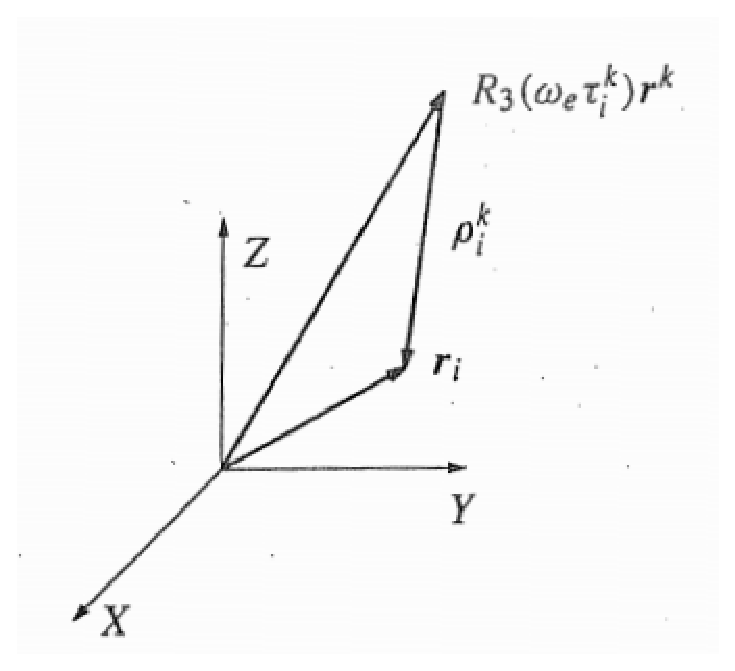
\includegraphics[width=0.7\linewidth]{TeX_files/Part03/chapter09/image/9-12}
		\caption{接收机坐标$r_i$在地心惯性坐标系和卫星坐标$R_3(\omega_e \tau ^k_i)r^k$在地心地固坐标系。 第一个位置是变成ECEF系统在z轴旋转的角度是$\omega_e \tau ^k_i$}
		\label{fig:9-12}
	\end{figure}
	
	根据星历表,所有卫星位置的计算在WGS-84坐标系钟,这是一个地心地固坐标系(ECEF)。这意味着我们必须旋转的卫星位置向量的三个轴向,相当于地球的角位移信号的传播从卫星到接收机。GPS卫星的高度约为20000公里。因此,信号传输时间是66ms。地球每自转$15arcsec$的角位移信号相当于地球的旋转轴的传播$1arcsec$。如果使用ECEF坐标并且没有调整,接收机坐标将偏向约相等于$1arcsec$的经度。
	
	依照图\ref{fig:9-12}卫星k和接收机i的距离对地球自转改正被定义为
	\begin{equation}\label{eq:9.17}
	\rho ^k_i = \Arrowvert R_3(\omega_e\tau^k_i)r^k(t-\tau^k_i)_{inert}-r_i(t)_{ECEF} \Arrowvert = 
	\Arrowvert \begin{bmatrix}
	X^k \\ Y^k \\ Z^k
	\end{bmatrix}-
	\begin{bmatrix}
	X_i \\ Y_i \\ Z_i
	\end{bmatrix} \Arrowvert
	\end{equation}
	
	矩阵$R_3$定义的旋转角度$\omega_e \tau^k_i$当信号传播时为:
	\begin{equation}\label{eq:9.18}
	R_3(\omega_e\tau^k_i) =
	\begin{bmatrix}
	\cos(\omega_e\tau^k_i) & \sin(\omega_e\tau^k_i) & 0 \\
	-\sin(\omega_e\tau^k_i) & \cos(\omega_e\tau^k_i) & 0 \\
	0 & 0 & 1
	\end{bmatrix}
	\end{equation}
	
	信号传播时间从(信号发出)卫星k到(信号接受)接收机i被表示为$\tau$。地球自转速率是$\omega_e$。ECEF系统中的位置向量表示为$r(t)_{ECEF}$。参数t强调对时间的依赖。
	
	伪距观测的基本方程的样子为:
	\begin{equation}\label{eq:9.19}
	P^k_i(t) = \rho^k_i+I^k_i+T^k_i-c(dt^k(t-\tau^k_i)-dt_i(t))-e^k_i
	\end{equation}
	
	电离层延迟为$I^k_i$,对流层延迟为$T^k_i$,c表示真空中的光速$e^k_i$表示一个错误。
	\begin{figure}
		\centering
		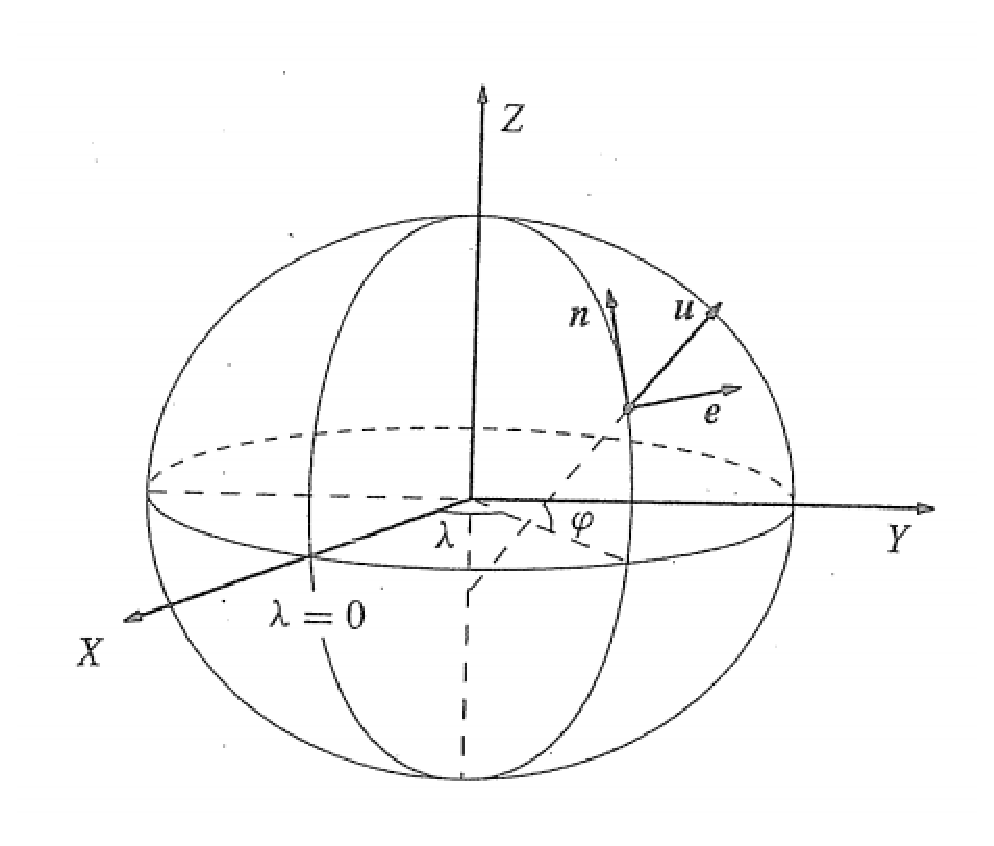
\includegraphics[width=0.7\linewidth]{TeX_files/Part03/chapter09/image/9-13}
		\caption{站心坐标系(e,n,u)}
		\label{fig:9-13}
	\end{figure}
	
	所以我们需要改变一个站心坐标系的向量x到当地的e,n坐标系,u为铅锤线方向,n指向北,e指向西,在图\ref{fig:9-13}中显示。 站心坐标系由地心矢量给出X,和三个单位向量的正交矩阵F已经介绍在(3.31)中介绍。
	\begin{equation}\label{eq:9.20}
	F = \begin{bmatrix}
	e & n & u
	\end{bmatrix}=
	\begin{bmatrix}
	-\sin \lambda & -\sin\varphi\cos\lambda & \cos\varphi\cos\lambda \\
	\cos \lambda & -\sin\varphi\sin\lambda & \cos\varphi\sin\lambda \\
	0 & \cos\varphi & \sin\varphi
	\end{bmatrix}
	\end{equation}
	
	知道笛卡尔坐标的初值$(X^0_i,Y^0_i,Z^0_i)$我们就可以计算接收机的地理坐标$(\varphi,\lambda)$,因此获得矩阵F。现在让$(E,N,U)=F^Tx$。我们立即获得方位角、高度角和距离:
	\begin{table}
		\begin{tabular}{ll}
			 方位角: 		 & $Az = \arctan(E/N)$ \\ 
			 高度角:		 & $El=\arctan(U/\sqrt{N^2+E^2})$ \\ 
			 距离: 		  & $s=\Arrowvert x \Arrowvert$ \\ 
		\end{tabular} 
	\end{table}
	
	知道高度角我们可以计算$T^k_i$。电离层延迟$I^k_i$设置为0,因为我们不知道更好的值,$dt^k$的值由式\ref{eq:9.16}计算得出。未知数$dt_i$和三维坐标$(X_i,Y_i,Z_i)$是隐藏在$\rho^k_i$。所以我们先线性化式\ref{eq:9.19}:
	\begin{equation}\label{eq:9.21}
	-\dfrac{X^k-X^0_i}{(\rho^k_i)^0}x_i-\dfrac{Y^k-Y^0_i}{(\rho^k_i)^0}y_i-\dfrac{Z^k-Z^0_i}{(\rho^k_i)^0}z_i+1(c\,dt_i)=(P^k_i)_{obs}-(P^k_i)^0-e^k_i=b_i-e^k_i
	\end{equation}
	
	第一个近似值我们设为 $\rho^k_i\approx(\rho^k_i)^0=(P^k_i)^0$,通过几何距离的近似值计算卫星和接收机的坐标。$b_i$表示观测值减去计算值。
	
	$(P^k_i)^0$的初值可能是源自或从可能的接收机的初步计算坐标$(X^0_i,Y^0_i,Z^0_i)$获得。这是修正接收机时钟偏移 $dt_i$,与第一个估计值$dt_i=0$。如果初值好则右侧$b_i$很小。注意方向余弦描述的参数使用式\ref{eq:9.17}。
	
	描述线性化观测方程的式子是\ref{eq:9.21}我们设置的未知数是$x=(x_i,y_i,z_i,c\,dt_i)$:
	\begin{equation}\label{eq:9.22}
	Ax=\begin{bmatrix}
	-\dfrac{X^1-X_i}{\rho^1_i} & -\dfrac{Y^1-Y_i}{\rho^1_i} & -\dfrac{Z^1-Z_i}{\rho^1_i} & 1 \\
	-\dfrac{X^2-X_i}{\rho^2_i} & -\dfrac{Y^2-Y_i}{\rho^2_i} & -\dfrac{Z^2-Z_i}{\rho^2_i} & 1 \\
	\vdots & & & \\
	-\dfrac{X^3-X_i}{\rho^3_i} & -\dfrac{Y^3-Y_i}{\rho^3_i} & -\dfrac{Z^3-Z_i}{\rho^3_i} & 1 \\
	\end{bmatrix}
	\begin{bmatrix}
	x_i \\ y_i \\ z_i \\ c\,dt_i
	\end{bmatrix}
	= b-e
	\end{equation}
	
	注意参数c和$dt_i$一起呆在在一个产品中。这样做是为了数值的原因。未知的$c\,dt_i$和另一未知数有着一样的维度,即长度。然而有些人喜欢随着时间估计。这可以通过使用未知的$dt_i$一起相当小系数$c x 10^9$收益率$dt_i$ns。???
	
	Row-wise包含前三列向量的方向余弦在卫星和接收机之间。最小二乘的解决方案是
	\begin{equation}\label{eq:9.23}
	\begin{bmatrix}
	\hat{x}_i \\ \hat{y}_i \\ \hat{z}_i \\ \widehat{c\,dt_i}
	\end{bmatrix}
	=(A^T\Sigma^{-1}A)^{-1}A^T\Sigma^{-1}b
	\end{equation}
	
	伪距观测值被认为是独立等效的方差$e\sim N(0,\sigma^2I)$。换句话说矢量e零均值和协方差矩阵$\Sigma=\sigma^2I$。如果这个假设是正确的,式\ref{eq:9.23}可以化简为
	\begin{equation}\label{eq:9.24}
	\begin{bmatrix}
	\hat{x}_i \\ \hat{y}_i \\ \hat{z}_i \\ \widehat{c\,dt_i}
	\end{bmatrix}
	=(A^TA)^{-1}A^Tb
	\end{equation}
	迭代接收机坐标
	\begin{equation}\label{eq:9.25}
	\hat{X}_i=X^0_i+\hat{x}_i,\quad \hat{Y}_i=Y^0_i+\hat{y}_i,\quad and \quad \hat{Z}_i=Z^0_i+\hat{z}_i,
	\end{equation}
	迭代涉及式\ref{eq:9.22},\ref{eq:9.24} 和 \ref{eq:9.25} 重复直到稳定 $\Arrowvert x\Arrowvert=\sqrt{x^Tx}$ 小于 $10^2$,可以说
	
	最后我们建立一个数据集组成的一个历元。它包含$PRN`s k = 1,4,7,13,20,24,25$在表\ref{tab:9.4}。伪距改正是根据以下方程:
	\begin{equation}\label{eq:9.26}
	P = observed\,pseudorange + c\,dt^k-T.
	\end{equation}
	
	M-文件easy3是调用satpos在传输时间的计算。
	\begin{table}
		\caption{坐标$(X^k,Y^k,Z^k)$ 卫星出现在一个特定的历元。观测到的伪距用$P^k$表示}
		\label{tab:9.4}
		\begin{tabular}{crrrr}
			\hline
			PRN & 1 & 4 & 7 & 13 \\ 
			\hline
			$X^k[m]$ & 14789533.14 &  11784778.93 &  20131229.62 & 22053478.89  \\ 
			$Y^k[m]$ &  7334543.20 & -10589833.27 & -17092167.32 & -4245955.78  \\ 
			$Z^k[m]$ & 20976503.11 &  21427005.76 &   1367264.01 & 14103264.45  \\ 
			$P^k[m]$ & 20589966.21 &  21428477.36 &  24767161.79 & 21266276.50  \\ 
			\hline
		\end{tabular} 
		\begin{tabular}{crrr}
			\hline
			PRN & 20 & 24 & 25 \\
			\hline
			$X^k[m]$ & 12654506.52 &  -1514708.63 & -9091147.00 \\
			$Y^k[m]$ & 17685295.10 & -16394944.97 & 13349830.35 \\ 
			$Z^k[m]$ & 15150460.02 &  21142855.83 & 21347346.61 \\ 
			$P^k[m]$ & 21871195.29 &  23851770.76 & 24109819.35 \\ 
			\hline
		\end{tabular}
	\end{table}	
	
	\begin{figure}
		\centering
		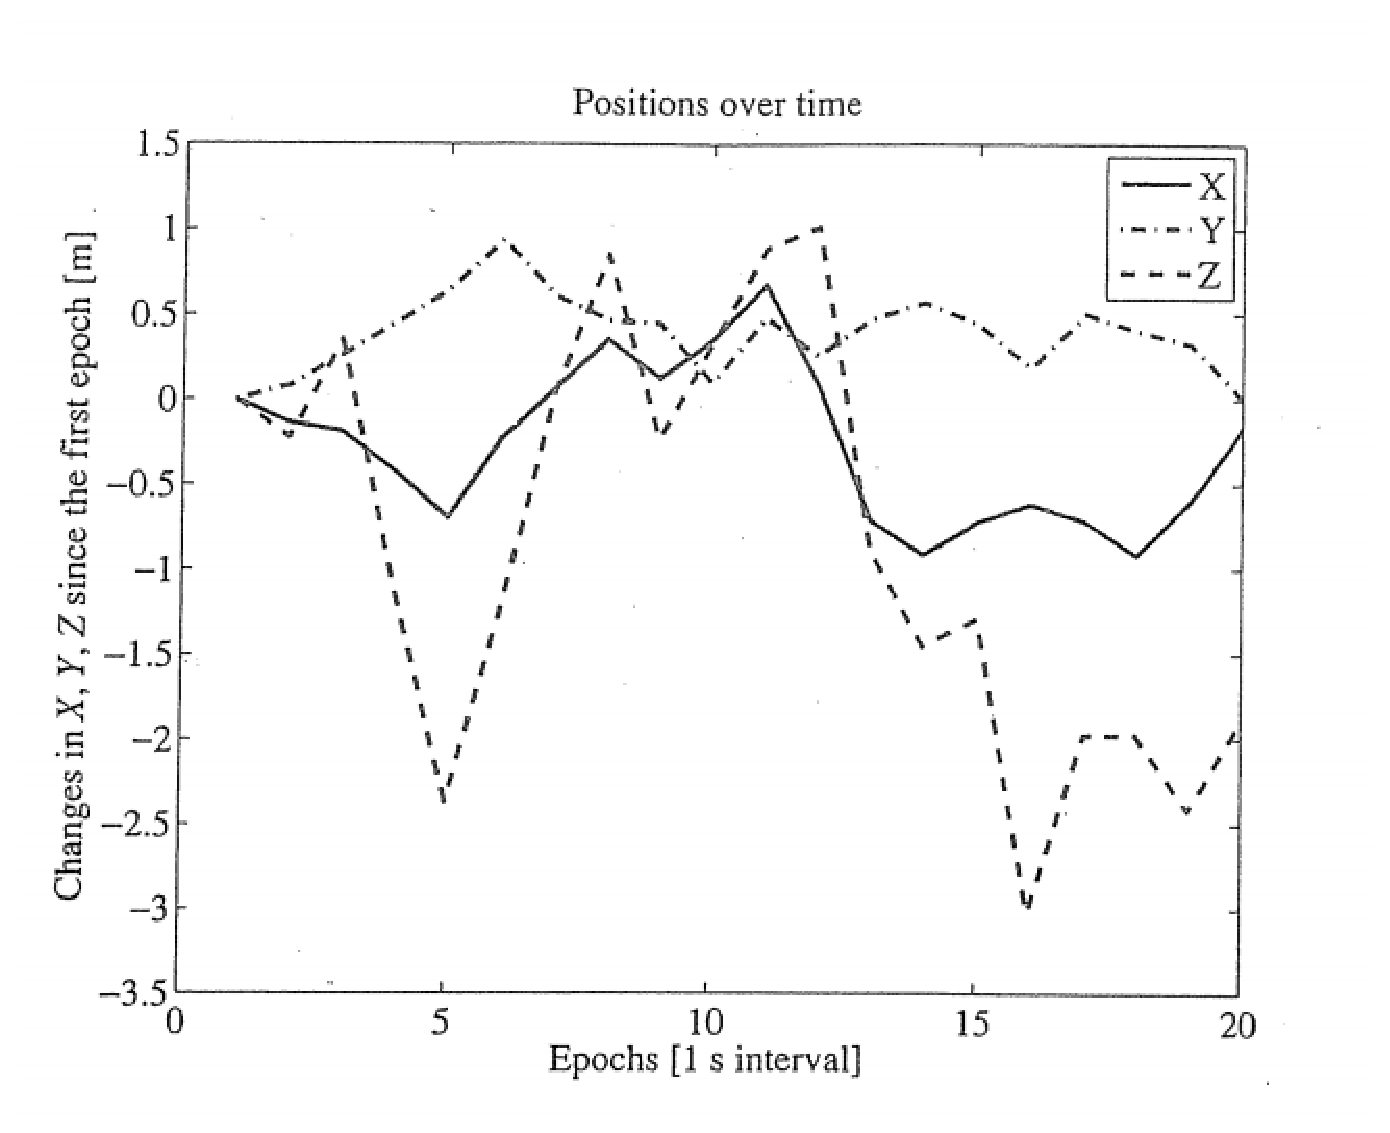
\includegraphics[width=0.7\linewidth]{TeX_files/Part03/chapter09/image/9-14}
		\caption{随时间变化由伪距得出的接收机坐标:X,Y,Z}
		\label{fig:9-14}
	\end{figure}
	
	知道卫星位置和测量的伪距我们可以估计接收机坐标和接收机时钟偏移量$\widehat{c\,dt}$通过最小二乘法:
	
	接收机的时钟偏移量和GPS时间相比为$\widehat{dt} = 0.377 ms$。6次迭代后得到的结果。接收机位置的标准差是2.3米,详见第四章。

	\subsection[例子3]{例子3\\easy3}\label{subsec:easy3}
		在easy3中我们通过O文件和N文件计算了接收机的ECEF坐标,仅仅使用了伪距值。GPST的传播时间是$(t_i-\tau^k_i)^{GPST}$ 用于计算卫星位置。
		
		接下来我们引用一个中心块的代码应用于任何位置计算。第一次可能很难阅读,但是我们试着把单词:目标是找到一个特定的历元在GPST从给定的卫星信号传播。我们知道历元 $t_i$、计算的接收机时钟,当观察值被确定。有信号传播$P/c$秒之前的卫星。我们知道了伪距P和光速c。接下来,我们计算的卫星时钟偏移tcorr参数$a_0$和$a_1$的星历表。然而,这个量取决于星历的时间发布在tOc。所以tcorr的值只能通过迭代,所以你看tcorr出现在左边的两倍。我们终于可以知道tcorr在那一刻计算的真实GPST信号传播时最后卫星的位置。代码如下:
		\begin{lstlisting}
		k = col_Eph(i);
		tx_RAW = time - obs(i)/v_light;
		tOc = Eph(21,k);
		dt = check_t(tx_RAW-tOc);
		tcorr = (Eph(2,k) * dt + Eph(20,k)) * dt + Eph(19,k);
		tx_GPS = tx_RAW- tcorr;
		dt - check_t(tx_GPS-tOc);
		tcorr = (Eph(2,k) * dt -f Eph(20,k)) * dt + Eph(19,k);
		tx_GPS = tx_RAW-tcorr;
		X = satpos(tx_GPS, Eph(:,k));			
		\end{lstlisting}
		下面的代码纠正地球自转导致的信号传播从卫星到接收机的误差。式\ref{eq:9.18}中描述卫星的位置必须在z轴旋转角$\omega_e\tau^k_i$。在第一个迭代中我们不知道确切的传播时间并将其设置为0.072秒。对流层延迟设置为0s。我们在下一次迭代估计卫星的仰角,作为这个角el计算对流层延迟是很重要的。它是实现对流层的代码。
		\begin{lstlisting}
		if iter == 1
			traveltime = 0.072;
			Rot_X = X;
			trop = 0;
		else
			rho2=(X(1)-pos(1))~2+(X(2)-pos(2))~2+(X(3)-pos(3))~2;
			traveltime = sqrt(rho2)/v_light;
			Rot_X = e_i'_corr(traveltime,X);
			rho2 = (Rot_X(l)-pos(1))^2 + (Rot_X(2)-pos(2))"2-r (Rot_X(3)-pos(3))^2;
			[az,el,dist] = topocent(pos(1:3 /:),Rot_X-pos(1:3,:));
			if iter == nojterations, El(i) = el; end
			trop=tropo(sin(el*dtr),0.0,1013.0,293.0,50.0,0.0,0.0,0.0);
		end
		\end{lstlisting}
		接收机的位置计算的关键代码是一个单独的m文件$recpo_ls$.
		
		我们打开一个RINEX格式的O文件读取所有的伪距。从easy2与给定的卫星位置,我们计算出接收机的位置。
		
		重复计算了20个历元。每个位置是迭代最小二乘的结果的过程。位置相对于第一个历元的变化如图\ref{fig:9-14}。坐标的变化值一般小于5米。
		
		
	

